\subsection{Ambito amministratore}

\hypertarget{A0}{}
\bookmark[dest=A0,level=3]{UCA 0: Caso base amministratore}
\subsubsection{UCA 0: Caso base amministratore}
\begin{figure}[H]
\centering
\includegraphics[trim=0cm 0.8cm 0cm 0cm,clip=true,scale=0.75]%
{./grafici/A0}
\caption{UCA 0: Caso base amministratore}
\end{figure}
\begin{itemize}
\item \textbf{Attori:} Amministratore;
\item \textbf{Descrizione:} L'amministratore può creare dei nuovi processi e gestire i processi creati;
\item \textbf{Precondizione:} Il sistema è attivo e l'amministratore ha iniziato ad interfacciarvisi;
\item \textbf{Scenario principale:}
\begin{itemize}
\item L'amministratore può creare un nuovo processo;
\item L'amministratore può gestire i processi creati.
\end{itemize}
%\item \textbf{Estensioni:}
%\item \textbf{Inclusioni:}
%\item \textbf{Scenario alternativo:}
\item \textbf{Postcondizione:} Il sistema ha eseguito e le operazioni effettuate dall'amministratore e ha salvato le modifiche sui processi.
\end{itemize}

\hypertarget{A1}{}
\bookmark[dest=A1,level=3]{UCA 1: Creazione di un nuovo processo}
\subsubsection{UCA 1: Creazione di un nuovo processo}
\begin{figure}[H]
\centering
\includegraphics[trim=0cm 0.8cm 0cm 0cm,clip=true,scale=0.75]%
{./grafici/A1}
\caption{UCA 1: Creazione di un nuovo processo}
\end{figure}
\begin{itemize}
\item \textbf{Attori:}
Amministratore;
\item \textbf{Descrizione:}
L'amministratore può creare un nuovo processo, gestirne i passi e definirne le condizioni di terminazione;
\item \textbf{Precondizione:} L'amministratore ha richiesto la creazione di un nuovo processo;
\item \textbf{Flusso principale degli eventi:}
\begin{enumerate}
\item L'amministratore può definire un nuovo processo;
\item L'amministratore può definire i criteri di terminazione del nuovo processo;
\item L'amministratore può gestire i passi del nuovo processo;
\item L'amministratore può avviare il processo.
\end{enumerate}
\item \textbf{Postcondizione:}
Il processo creato dall'utente è stato avviato e salvato dal sistema che ritorna allo stato iniziale.
\end{itemize}

\hypertarget{A1.1}{}
\bookmark[dest=A1.1,level=4]{UCA 1.1: Definizione di un nuovo processo}
\subsubsection{UCA 1.1: Definizione di un nuovo processo}
\begin{figure}[H]
\centering
\includegraphics[trim=0cm 0.8cm 0cm 0cm,clip=true,scale=0.75]%
{./grafici/A11}
\caption{UCA 1.1: Definizione di un nuovo processo}
\end{figure}
\begin{itemize}
\item \textbf{Attori:}
Amministratore;
\item \textbf{Descrizione:}
L'amministratore può creare un nuovo processo definendone il nome, che deve essere univoco, e la descrizione;
\item \textbf{Precondizione:} L'amministratore ha richiesto la creazione di un nuovo processo;
\item \textbf{Flusso principale degli eventi:}
\begin{enumerate}
\item L'amministratore inserisce il nome del processo;
\item L'amministratore inserisce la descrizione del processo.
\end{enumerate}
\item \textbf{Scenario alternativo:}
\begin{itemize}
\item Il nome inserito è già stato scelto per un altro processo, perciò l'amministratore viene avvisato e può cambiare i dati immessi;
\end{itemize}
\item \textbf{Postcondizione:}
La definizione del processo è stata inserita e il sistema continua con la procedura di creazione del processo.
\end{itemize}

\hypertarget{A1.1.1}{}
\bookmark[dest=A1.1.1,level=4]{UCA 1.1.1: Inserimento del nome del processo}
\subsubsection{UCA 1.1.1: Inserimento del nome del processo}
\begin{itemize}
\item \textbf{Attori:}
Amministratore;
\item \textbf{Descrizione:}
L'amministratore può inserire un nome per il nuovo processo in creazione;
\item \textbf{Precondizione:}
L'amministratore ha richiesto la creazione di un nuovo processo e vuole inserire il nome scelto;
\item \textbf{Postcondizione:}
Il nome del processo è stato inserito e il sistema continua la procedura di creazione del nuovo processo.
\end{itemize}

\hypertarget{A1.1.2}{}
\bookmark[dest=A1.1.2,level=4]{UCA 1.1.2: Inserimento della descrizione del processo}
\subsubsection{UCA 1.1.2: Inserimento della descrizione del processo}

\begin{itemize}
\item \textbf{Attori:}
Amministratore;
\item \textbf{Descrizione:}
L'amministratore può inserire una descrizione per il nuovo processo in creazione;
\item \textbf{Precondizione:}
L'amministratore ha richiesto la creazione di un nuovo processo e vuole inserire la descrizione;
\item \textbf{Postcondizione:}
La descrizione del processo è stata inserita e il sistema continua la procedura di creazione del nuovo processo.
\end{itemize}

\hypertarget{A1.2}{}
\bookmark[dest=A1.2,level=4]{UCA 1.2: Definizione dei criteri di terminazione del processo}
\subsubsection{UCA 1.2: Definizione dei criteri di terminazione del processo}
\begin{figure}[H]
\centering
\includegraphics[trim=0cm 0.8cm 0cm 0cm,clip=true,scale=0.75]%
{./grafici/A12}
\caption{UCA 1.2: Definizione dei criteri di terminazione del processo}
\end{figure}
\begin{itemize}
\item \textbf{Attori:}
Amministratore;
\item \textbf{Descrizione:}
L'amministratore può scegliere i criteri di terminazione del processo in definizione.
Questi criteri sono il completamento del processo da parte di un certo numero di utenti ed eventualmente una precisa data di scadenza;
\item \textbf{Precondizione:}
L'amministratore vuole definire i criteri di terminazione del processo in creazione;
\item \textbf{Scenario principale:}
\begin{itemize}
\item L'amministratore può scegliere il numero di completamenti che causano la terminazione del processo;
\item L'amministratore può scegliere la data di scadenza del processo.
\end{itemize}
\item \textbf{Postcondizione:}
I criteri di terminazione sono stati inseriti e il sistema continua con la procedura di creazione del processo.
\end{itemize}

\hypertarget{A1.2.1}{}
\bookmark[dest=A1.2.1,level=4]{UCA 1.2.1: Scelta del massimo numero possibile di completamenti del processo}
\subsubsection{UCA 1.2.1: Scelta del massimo numero possibile di completamenti del processo}

\begin{itemize}
\item \textbf{Attori:}
Amministratore;
\item \textbf{Descrizione:}
L'amministratore può scegliere il numero di completamenti del processo da parte degli utenti, necessario e sufficiente a causarne la terminazione;
\item \textbf{Precondizione:}
L'amministratore vuole definire il massimo numero possibile di completamenti del processo in creazione;
\item \textbf{Postcondizione:}
Il massimo numero possibile di completamenti del processo in creazione è stato inserito e il sistema continua con la definizione dei criteri di terminazione.
\end{itemize}

\hypertarget{A1.2.2}{}
\bookmark[dest=A1.2.2,level=4]{UCA 1.2.2: Scelta della data di scadenza del processo}
\subsubsection{UCA 1.2.2: Scelta della data di scadenza del processo}

\begin{itemize}
\item \textbf{Attori:}
Amministratore;
\item \textbf{Descrizione:}
L'amministratore può scegliere la data di terminazione del processo;
\item \textbf{Precondizione:}
L'amministratore vuole definire la data di scadenza del processo in creazione;
\item \textbf{Postcondizione:}
La data di scadenza del processo in creazione è stato inserita e il sistema continua con la definizione dei criteri di terminazione.
\end{itemize}

\hypertarget{A1.3}{}
\bookmark[dest=A1.3,level=4]{UCA 1.3: Gestione dei passi del processo}
\subsubsection{UCA 1.3: Gestione dei passi del processo}
\begin{figure}[H]
\centering
\includegraphics[trim=0cm 0.8cm 0cm 0cm,clip=true,scale=0.75]%
{./grafici/A13}
\caption{UCA 1.3: Gestione dei passi del processo}
\end{figure}
\begin{itemize}
\item \textbf{Attori:}
Amministratore;
\item \textbf{Descrizione:}
L'amministratore può creare un nuovo passo oppure gestire i passi creati;
\item \textbf{Precondizione:}
L'amministratore ha definito un nuovo processo e vuole gestirne i passi;
\item \textbf{Scenario principale:}
\begin{itemize}
\item L'amministratore può creare un nuovo passo;
\item L'amministratore può visualizzare la lista dei passi creati;
\item L'amministratore può modificare un passo creato;
\item L'amministratore può eliminare un passo creato.
\end{itemize}
\item \textbf{Postcondizione:}
Il sistema ha eseguito e salvato le operazioni effettuate dall'amministratore sui passi del processo in creazione e il sistema è pronto per avviarlo.
\end{itemize}

\hypertarget{A1.3.1}{}
\bookmark[dest=A1.3.1,level=4]{UCA 1.3.1: Creazione di un passo}
\subsubsection{UCA 1.3.1: Creazione di un passo}
\begin{figure}[H]
\centering
\includegraphics[trim=0cm 0.8cm 0cm 0cm,clip=true,scale=0.75]%
{./grafici/A131}
\caption{UCA 1.3.1: Creazione di un passo}
\end{figure}
\begin{itemize}
\item \textbf{Attori:}
Amministratore;
\item \textbf{Descrizione:}
L'amministratore può aggiungere un nuovo passo al processo in creazione definendone i dati, i vincoli di superamento, e una descrizione;
\item \textbf{Precondizione:}
L'amministratore vuole aggiungere un nuovo passo al processo in creazione;
\item \textbf{Scenario principale:}
\begin{itemize}
\item L'amministratore inserisce la descrizione del passo;
\item L'amministratore inserisce uno o più dati al passo;
\item L'amministratore può inserire uno o più criteri di superamento del passo.
\end{itemize}
\item \textbf{Postcondizione:}
Il sistema ha aggiunto il passo definito dall'utente al processo in creazione.
\end{itemize}

\hypertarget{A1.3.1.1}{}
\bookmark[dest=A1.3.1.1,level=4]{UCA 1.3.1.1: Inserimento della descrizione del passo}
\subsubsection{UCA 1.3.1.1: Inserimento della descrizione del passo}
\begin{itemize}
\item \textbf{Attori:}
Amministratore;
\item \textbf{Descrizione:}
L'amministratore può inserire la descrizione del passo in creazione, per definirne lo scopo;
\item \textbf{Precondizione:}
L'amministratore vuole inserire la descrizione del passo in creazione;
\item \textbf{Postcondizione:}
La descrizione del passo è stata inserita e il sistema prosegue con la creazione del passo.
\end{itemize}

\hypertarget{A1.3.1.2}{}
\bookmark[dest=A1.3.1.2,level=4]{UCA 1.3.1.2: Inserimento dei dati del passo}
\subsubsection{UCA 1.3.1.2: Inserimento dei dati del passo}
\begin{figure}[H]
\centering
\includegraphics[trim=0cm 0.8cm 0cm 0cm,clip=true,scale=0.75]%
{./grafici/A1312}
\caption{UCA 1.3.1.2: Inserimento dei dati del passo}
\end{figure}
\begin{itemize}
\item \textbf{Attori:}
Amministratore;
\item \textbf{Descrizione:}
L'amministratore può aggiungere uno o più campi dati al passo in creazione, scegliendone il nome e il tipo;
\item \textbf{Precondizione:}
L'amministratore vuole aggiungere un campo dati al passo in creazione;
\item \textbf{Scenario principale:}
\begin{itemize}
\item L'amministratore inserisce il nome del dato;
\item L'amministratore seleziona il tipo del dato.
\end{itemize}
\item \textbf{Postcondizione:}
Il dato scelto è stato inserito e il sistema prosegue con la creazione del passo.
\end{itemize}

\hypertarget{A1.3.1.2.1}{}
\bookmark[dest=A1.3.1.2.1,level=4]{UCA 1.3.1.2.1: Inserimento del nome del dato}
\subsubsection{UCA 1.3.1.2.1: Inserimento del nome del dato}
\begin{itemize}
\item \textbf{Attori:}
Amministratore;
\item \textbf{Descrizione:}
L'amministratore può inserire il nome del campo dati del passo in creazione, per chiarirne il significato;
\item \textbf{Precondizione:}
L'amministratore vuole aggiungere il nome del campo dati aggiunto al passo in creazione;
\item \textbf{Postcondizione:}
Il nome del dato aggiunto è stato inserito e il sistema prosegue con la definizione del dato del passo in creazione.
\end{itemize}

\hypertarget{A1.3.1.2.2}{}
\bookmark[dest=A1.3.1.2.2,level=4]{UCA 1.3.1.2.2: Selezione del tipo del dato}
\subsubsection{UCA 1.3.1.2.2: Selezione del tipo del dato}
\begin{itemize}
\item \textbf{Attori:}
Amministratore;
\item \textbf{Descrizione:}
L'amministratore può scegliere se il tipo di dato da aggiungere deve essere testuale, numerico o un'immagine;
\item \textbf{Precondizione:}
L'amministratore vuole aggiungere un campo dati al passo in creazione;
\item \textbf{Postcondizione:}
Il tipo del dato aggiunto è stato inserito e il sistema prosegue con la definizione del dato del passo in creazione.
\end{itemize}

\hypertarget{A1.3.1.3}{}
\bookmark[dest=A1.3.1.3,level=4]{UCA 1.3.1.3: Definizione di un criterio di superamento del passo}
\subsubsection{UCA 1.3.1.3: Definizione di un criterio di superamento del passo}
\begin{figure}[H]
\centering
\includegraphics[trim=0cm 0.8cm 0cm 0cm,clip=true,scale=0.75]%
{./grafici/A1313}
\caption{UCA 1.3.1.3: Definizione di un criterio di superamento del passo}
\end{figure}
\begin{itemize}
\item \textbf{Attori:}
Amministratore;
\item \textbf{Descrizione:}
L'amministratore può definire uno o più criteri di superamento del passo in creazione.
Per ciascun criterio può stabilire delle condizioni, e il passo eseguibile dopo il loro soddisfacimento.
I vincoli di ciascun criterio devono essere disgiunti per non creare ambiguità sul successivo passo da eseguire: eventuali errori vengono notificati dall'amministratore che potrà correggere i dati immessi;
\item \textbf{Precondizione:}
L'amministratore vuole aggiungere un criterio di superamento del passo in creazione;
\item \textbf{Flusso principale degli eventi:}
\begin{enumerate}
\item L'amministratore definisce le condizioni di avanzamento;
\item L'amministratore definisce il passo eseguibile al soddisfacimento delle condizioni scelte.
\end{enumerate}
\item \textbf{Scenario alternativo:}
\begin{itemize}
\item Le condizioni definite non sono disgiunte da quelle inserite in altri criteri di superamento, quindi l'utente viene avvisato dell'errore e può correggere i vincoli inseriti;
\item Tra le condizioni di avanzamento definite è stata scelta la possibilità di saltare il passo, ma esiste già un criterio di superamento che lo permette. L'utente viene avvisato dell'errore e può correggere i vincoli inseriti.
\end{itemize}
\item \textbf{Postcondizione:}
Il criterio di superamento definito dall'amministratore è stato aggiunto e il sistema prosegue con la creazione del passo.
\end{itemize}

\hypertarget{A1.3.1.3.1}{}
\bookmark[dest=A1.3.1.3.1,level=4]{UCA 1.3.1.3.1: Inserimento delle condizioni di avanzamento}
\subsubsection{UCA 1.3.1.3.1: Inserimento delle condizioni di avanzamento}
\begin{figure}[H]
\centering
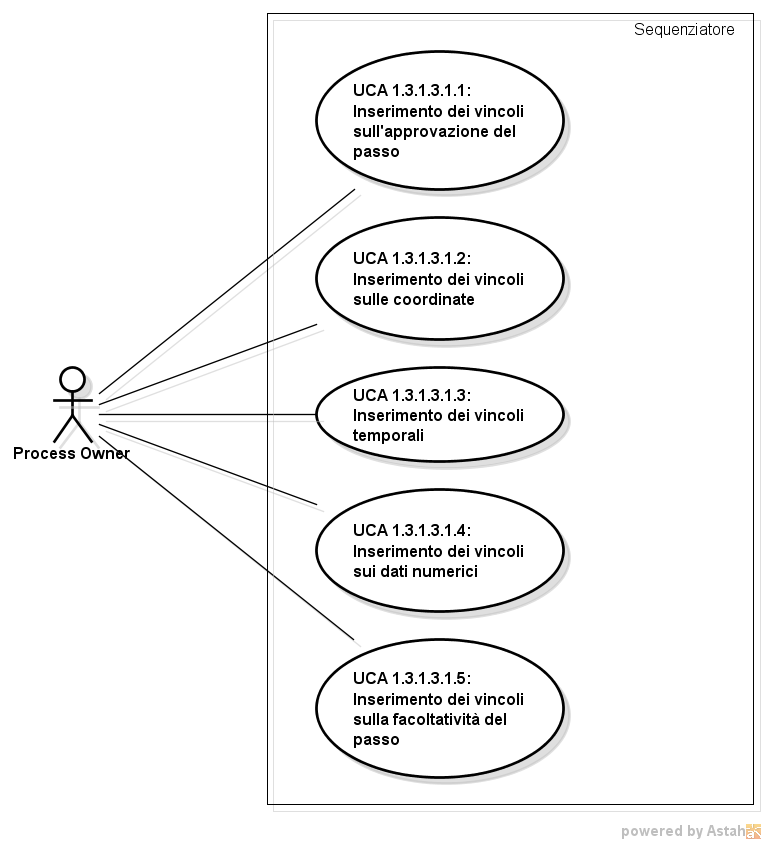
\includegraphics[trim=0cm 0.8cm 0cm 0cm,clip=true,width=%
\textwidth]
{./grafici/A13131}
\caption{UCA 1.3.1.3.1: Inserimento delle condizioni di avanzamento}
\end{figure}
\begin{itemize}
\item \textbf{Attori:}
Amministratore;
\item \textbf{Descrizione:}
L'amministratore può decidere le condizioni che determinano il criterio di superamento in definizione.
Può inserire delle condizioni sull'approvazione e sulla facoltatività del passo, sui dati numerici, e sulla data, l'ora e la posizione geografica dell'utente al momento dell'invio dei dati richiesti.
\item \textbf{Precondizione:}
L'amministratore sta definendo un nuovo criterio di superamento del passo in creazione;
\item \textbf{Scenario principale:}
\begin{itemize}
\item L'amministratore può definire i vincoli sull'approvazione del passo;
\item L'amministratore può definire i vincoli sulle coordinate;
\item L'amministratore può definire i vincoli temporali;
\item L'amministratore può definire i vincoli sui dati numerici;
\item L'amministratore può definire i vincoli sulla facoltatività del passo.
\end{itemize}
\item \textbf{Postcondizione:}
Le condizioni definite dall'amministratore sono state aggiunte e il sistema prosegue con la definizione del criterio di superamento del passo.
\end{itemize}

\hypertarget{A1.3.1.3.1.1}{}
\bookmark[dest=A1.3.1.3.1.1,level=4]{UCA 1.3.1.3.1.1: Inserimento dei vincoli sull'approvazione del passo}
\subsubsection{UCA 1.3.1.3.1.1: Inserimento dei vincoli sull'approvazione del passo}
\begin{itemize}
\item \textbf{Attori:}
Amministratore;
\item \textbf{Descrizione:}
L'amministratore può decidere se per soddisfare il criterio di superamento in definizione, i dati inviati dall'utente necessiteranno dell'approvazione dell'amministratore;
\item \textbf{Precondizione:}
L'amministratore vuole definire i vincoli sull'approvazione del passo in creazione;
\item \textbf{Postcondizione:}
I vincoli sull'approvazione del passo sono stati inseriti e il sistema prosegue con la definizione del criterio di superamento del passo.
\end{itemize}

\hypertarget{A1.3.1.3.1.2}{}
\bookmark[dest=A1.3.1.3.1.2,level=4]{UCA 1.3.1.3.1.2: Inserimento dei vincoli sulle coordinate}
\subsubsection{UCA 1.3.1.3.1.2: Inserimento dei vincoli sulle coordinate}
\begin{itemize}
\item \textbf{Attori:}
Amministratore;
\item \textbf{Descrizione:}
L'amministratore può inserire i vincoli sulla posizione dell'utente al momento dell'invio dei dati, stabilendo le coordinate del luogo in cui dovrà trovarsi e un'eventuale raggio di tolleranza;
\item \textbf{Precondizione:}
L'amministratore vuole definire i vincoli sulle coordinate dell'utente al momento dell'invio dei dati;
\item \textbf{Postcondizione:}
I vincoli sulle coordinate dell'utente sono stati inseriti e il sistema prosegue con la definizione del criterio di superamento del passo.
\end{itemize}

\hypertarget{A1.3.1.3.1.3}{}
\bookmark[dest=A1.3.1.3.1.3,level=4]{UCA 1.3.1.3.1.3: Inserimento dei vincoli temporali}
\subsubsection{UCA 1.3.1.3.1.3: Inserimento dei vincoli temporali}
\begin{itemize}
\item \textbf{Attori:}
Amministratore;
\item \textbf{Descrizione:}
L'amministratore può inserire uno o più intervalli temporali in cui l'utente può inviare i dati;
\item \textbf{Precondizione:}
L'amministratore vuole definire i vincoli temporali sull'invio dei dati;
\item \textbf{Postcondizione:}
I vincoli temporali sull'invio dei dati sono stati inseriti e il sistema prosegue con la definizione del criterio di superamento del passo.
\end{itemize}

\hypertarget{A1.3.1.3.1.4}{}
\bookmark[dest=A1.3.1.3.1.4,level=4]{UCA 1.3.1.3.1.4: Inserimento dei vincoli sui dati numerici}
\subsubsection{UCA 1.3.1.3.1.4: Inserimento dei vincoli sui dati numerici}
\begin{itemize}
\item \textbf{Attori:}
Amministratore;
\item \textbf{Descrizione:}
L'amministratore può inserire i vincoli sui dati numerici che possono essere il numero di cifre, la possibilità di inserire cifre decimali o meno, e un eventuale limite superiore o inferiore;
\item \textbf{Precondizione:}
Esiste almeno un dato numerico nel passo in creazione e l'amministratore vuole definirne i vincoli;
\item \textbf{Postcondizione:}
I vincoli sui dati numerici del passo sono stati inseriti e il sistema prosegue con la definizione del criterio di superamento del passo.
\end{itemize}

\hypertarget{A1.3.1.3.1.5}{}
\bookmark[dest=A1.3.1.3.1.5,level=4]{UCA 1.3.1.3.1.5: Inserimento dei vincoli sulla facoltatività del passo}
\subsubsection{UCA 1.3.1.3.1.5: Inserimento dei vincoli sulla facoltatività del passo}
\begin{itemize}
\item \textbf{Attori:}
Amministratore;
\item \textbf{Descrizione:}
L'amministratore può decidere se l'utente potrà decidere di saltare il passo in creazione;
\item \textbf{Precondizione:}
L'amministratore vuole definire i vincoli sulla facoltatività del passo in creazione;
\item \textbf{Postcondizione:}
I vincoli sulla facoltatività del passo sono stati inseriti e il sistema prosegue con la definizione del criterio di superamento del passo.
\end{itemize}

\hypertarget{A1.3.1.3.2}{}
\bookmark[dest=A1.3.1.3.2,level=4]{UCA 1.3.1.3.2: Definizione passo successivo}
\subsubsection{UCA 1.3.1.3.2: Definizione passo successivo}
\begin{itemize}
\item \textbf{Attori:}
Amministratore;
\item \textbf{Descrizione:}
L'amministratore può definire il passo eseguibile al soddisfacimento dei vincoli scelti. Tra tutti i passi creati può scegliere solo quelli da cui è impossibile ritornare al passo in creazione, oppure la fine del processo;
\item \textbf{Precondizione:}
L'amministratore sta definendo un nuovo criterio di avanzamento e vuole stabilire il passo successivo al passo in creazione;
\item \textbf{Postcondizione:}
Il passo raggiungibile soddisfacendo i criteri di avanzamento in definizione è stato aggiunto.
\end{itemize}

\hypertarget{A1.3.2}{}
\bookmark[dest=A1.3.2,level=4]{UCA 1.3.2: Visualizzazione della lista dei passi creati}
\subsubsection{UCA 1.3.2: Visualizzazione della lista dei passi creati}
\begin{itemize}
\item \textbf{Attori:}
Amministratore;
\item \textbf{Descrizione:}
L'amministratore può visualizzare la lista, eventualmente vuota, dei passi creati;
\item \textbf{Precondizione:}
L'amministratore sta gestendo i passi del processo in creazione;
\item \textbf{Postcondizione:}
Il sistema ha visualizzato la lista dei passi creati.
\end{itemize}

\hypertarget{A1.3.3}{}
\bookmark[dest=A1.3.3,level=4]{UCA 1.3.3: Modifica di un passo}
\subsubsection{UCA 1.3.3: Modifica di un passo}
\begin{figure}[H]
\centering
\includegraphics[trim=0cm 0.8cm 0cm 0cm,clip=true,scale=0.75]%
{./grafici/A133}
\caption{UCA 1.3.3: Modifica di un passo}
\end{figure}
\begin{itemize}
\item \textbf{Attori:}
Amministratore;
\item \textbf{Descrizione:}
L'amministratore può modificare un passo creato. In particolare può modificarne la descrizione, il nome dei dati e i criteri di superamento;
\item \textbf{Precondizione:}
L'amministratore vuole modificare un passo dalla lista dei passi creati;
\item \textbf{Scenario principale:}
\begin{itemize}
\item L'amministratore può modificare la descrizione del passo;
\item L'amministratore può modificare la descrizione dei dati del passo;
\item L'amministratore può modificare i criteri di superamento del passo.
\end{itemize}
\item \textbf{Postcondizione:}
Le modifiche effettuate dall'amministratore sul passo creato sono state eseguite e il sistema ritorna alla gestione dei passi del processo.
\end{itemize}

\hypertarget{A1.3.3.1}{}
\bookmark[dest=A1.3.3.1,level=4]{UCA 1.3.3.1: Modifica della descrizione di un passo}
\subsubsection{UCA 1.3.3.1: Modifica della descrizione di un passo}
\begin{itemize}
\item \textbf{Attori:}
Amministratore;
\item \textbf{Descrizione:}
L'amministratore può inserire una nuova la descrizione di un passo creato;
\item \textbf{Precondizione:}
L'amministratore vuole modificare la descrizione di un passo creato;
\item \textbf{Postcondizione:}
La nuova descrizione è stata inserita e il sistema prosegue con la modifica del passo gestito.
\end{itemize}

\hypertarget{A1.3.3.2}{}
\bookmark[dest=A1.3.3.2,level=4]{UCA 1.3.3.2: Modifica della descrizione dei dati di un passo}
\subsubsection{UCA 1.3.3.2: Modifica della descrizione dei dati di un passo}
\begin{itemize}
\item \textbf{Attori:}
Amministratore;
\item \textbf{Descrizione:}
L'amministratore può inserire una nuova descrizione ai dati di un passo creato;
\item \textbf{Precondizione:}
L'amministratore vuole modificare la descrizione di un passo creato;
\item \textbf{Postcondizione:}
La nuova descrizione è stata inserita e il sistema prosegue con la modifica del passo gestito.
\end{itemize}

\hypertarget{A1.3.3.3}{}
\bookmark[dest=A1.3.3.3,level=4]{UCA 1.3.3.3: Modifica dei criteri di superamento di un passo}
\subsubsection{UCA 1.3.3.3: Modifica dei criteri di superamento di un passo}
\begin{figure}[H]
\centering
\includegraphics[trim=0cm 0.8cm 0cm 0cm,clip=true,scale=0.75]%
{./grafici/A1333}
\caption{UCA 1.3.3.3: Modifica dei criteri di superamento di un passo}
\end{figure}
\begin{itemize}
\item \textbf{Attori:}
Amministratore;
\item \textbf{Descrizione:}
L'amministratore può modificare uno o più criteri di superamento del passo gestito.
Per ciascun criterio può modificare le condizioni di avanzamento, e il passo eseguibile dopo il loro soddisfacimento.
I vincoli di ciascun criterio, dopo la modifica, devono essere disgiunti per non creare ambiguità sul successivo passo da eseguire: eventuali
errori vengono notificati dall'amministratore che potrà correggere i dati immessi;
\item \textbf{Precondizione:}
L'amministratore vuole modificare un criterio di superamento del passo gestito;
\item \textbf{Scenario principale:}
\begin{itemize}
\item L'amministratore può modificare le condizioni di avanzamento del passo;
\item L'amministratore può modificare il passo eseguibile al soddisfacimento delle condizioni scelte.
\end{itemize}
\item \textbf{Scenario alternativo:}
\begin{itemize}
\item Le condizioni definite non sono disgiunte dalle altre condizioni presenti, quindi l'utente viene avvisato dell'errore e può correggere i vincoli modificati;
\item Tra le condizioni di avanzamento definite è stata scelta la possibilità di saltare il passo, ma esiste già un criterio di superamento che lo permette. L'utente viene avvisato dell'errore e può correggere i vincoli modificati.
\end{itemize}
\item \textbf{Postcondizione:}
Le modifiche effettuate dall'amministratore sui criteri di superamento del passo gestito sono state eseguite e il sistema prosegue con la modifica del passo.
\end{itemize}

\hypertarget{A1.3.3.3.1}{}
\bookmark[dest=A1.3.3.3.1,level=4]{UCA 1.3.3.3.1: Modifica delle condizioni di avanzamento}
\subsubsection{UCA 1.3.3.3.1: Modifica delle condizioni di avanzamento}
\begin{figure}[H]
\centering
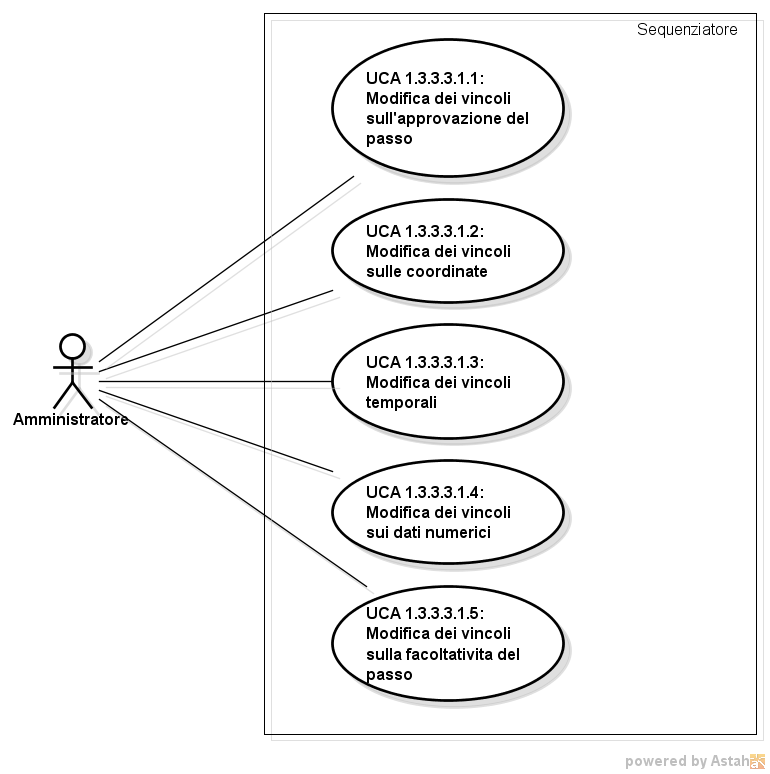
\includegraphics[trim=0cm 0.8cm 0cm 0cm,clip=true,width=%
\textwidth]
{./grafici/A13331}
\caption{UCA 1.3.3.3.1: Modifica delle condizioni di avanzamento}
\end{figure}
\begin{itemize}
\item \textbf{Attori:}
Amministratore;
\item \textbf{Descrizione:}
L'amministratore può modificare le condizioni che determinano il criterio di superamento in definizione.
Può modificare le condizioni sull'approvazione e la facoltatività del passo, sui dati numerici, e sulla data, l'ora e la posizione geografica dell'utente al momento dell'invio dei dati richiesti.
\item \textbf{Precondizione:}
L'amministratore vuole modificare le condizioni di avanzamento del passo gestito;
\item \textbf{Scenario principale:}
\begin{itemize}
\item L'amministratore può modificare i vincoli sull'approvazione del passo;
\item L'amministratore può modificare i vincoli sulle coordinate;
\item L'amministratore può modificare i vincoli temporali;
\item L'amministratore può modificare i vincoli sui dati numerici;
\item L'amministratore può modificare i vincoli sulla facoltatività.
\end{itemize}
\item \textbf{Postcondizione:}
Le modifiche effettuate dall'amministratore sulle condizioni di avanzamento del passo gestito sono state eseguite e il sistema prosegue con la modifica dei criteri di superamento.
\end{itemize}

\hypertarget{A1.3.3.3.1.1}{}
\bookmark[dest=A1.3.3.3.1.1,level=4]{UCA 1.3.3.3.1.1: Modifica dei vincoli sull'approvazione del passo}
\subsubsection{UCA 1.3.3.3.1.1: Modifica dei vincoli sull'approvazione del passo}
\begin{itemize}
\item \textbf{Attori:}
Amministratore;
\item \textbf{Descrizione:}
L'amministratore può modificare i vincoli sull'approvazione del passo;
\item \textbf{Precondizione:}
L'amministratore vuole modificare i vincoli sull'approvazione del passo gestito;
\item \textbf{Postcondizione:}
I vincoli sull'approvazione del passo sono stati modificati e il sistema prosegue con la modifica del criterio di superamento del passo.
\end{itemize}

\hypertarget{A1.3.3.3.1.2}{}
\bookmark[dest=A1.3.3.3.1.2,level=4]{UCA 1.3.3.3.1.2: Modifica dei vincoli sulle coordinate}
\subsubsection{UCA 1.3.3.3.1.2: Modifica dei vincoli sulle coordinate}
\begin{itemize}
\item \textbf{Attori:}
Amministratore;
\item \textbf{Descrizione:}
L'amministratore può modificare i vincoli sulla posizione dell'utente al momento dell'invio dei dati, stabilendo le coordinate del luogo in cui dovrà trovarsi e un'eventuale raggio di tolleranza;
\item \textbf{Precondizione:}
L'amministratore vuole modificare i vincoli sulle coordinate dell'utente al momento dell'invio dei dati;
\item \textbf{Postcondizione:}
I vincoli sulle coordinate dell'utente sono stati modificati e il sistema prosegue con la modifica del criterio di superamento del passo.
\end{itemize}

\hypertarget{A1.3.3.3.1.3}{}
\bookmark[dest=A1.3.3.3.1.3,level=4]{UCA 1.3.3.3.1.3: Modifica dei vincoli temporali}
\subsubsection{UCA 1.3.3.3.1.3: Modifica dei vincoli temporali}
\begin{itemize}
\item \textbf{Attori:}
Amministratore;
\item \textbf{Descrizione:}
L'amministratore può modificare gli intervalli temporali in cui l'utente può inviare i dati;
\item \textbf{Precondizione:}
L'amministratore vuole modificare i vincoli temporali sull'invio dei dati;
\item \textbf{Postcondizione:}
I vincoli temporali sull'invio dei dati sono stati modificati e il sistema prosegue con la modifica del criterio di superamento del passo.
\end{itemize}

\hypertarget{A1.3.3.3.1.4}{}
\bookmark[dest=A1.3.3.3.1.4,level=4]{UCA 1.3.3.3.1.4: Modifica dei vincoli sui dati numerici}
\subsubsection{UCA 1.3.3.3.1.4: Modifica dei vincoli sui dati numerici}
\begin{itemize}
\item \textbf{Attori:}
Amministratore;
\item \textbf{Descrizione:}
L'amministratore può modificare i vincoli sui dati numerici del passo gestito;
\item \textbf{Precondizione:}
Esiste almeno un dato numerico nel passo gestito e l'amministratore vuole modificarne i vincoli;
\item \textbf{Postcondizione:}
I vincoli sui dati numerici del passo sono stati modificati e il sistema prosegue con la modifica del criterio di superamento del passo.
\end{itemize}

\hypertarget{A1.3.3.3.1.5}{}
\bookmark[dest=A1.3.3.3.1.5,level=4]{UCA 1.3.3.3.1.5: Modifica dei vincoli sulla facoltatività del passo}
\subsubsection{UCA 1.3.3.3.1.5: Modifica dei vincoli sulla facoltatività del passo}
\begin{itemize}
\item \textbf{Attori:}
Amministratore;
\item \textbf{Descrizione:}
L'amministratore può modificare i vincoli sulla facoltatività del passo gestito;
\item \textbf{Precondizione:}
L'amministratore vuole modificare i vincoli sulla facoltatività del passo in gestione;
\item \textbf{Postcondizione:}
I vincoli sulla facoltatività del passo sono stati modificati e il sistema prosegue con la definizione del criterio di superamento del passo.
\end{itemize}

\hypertarget{A1.3.3.3.2}{}
\bookmark[dest=A1.3.3.3.2,level=4]{UCA 1.3.3.3.2: Modifica del passo successivo}
\subsubsection{UCA 1.3.3.3.2: Modifica del passo successivo}
\begin{itemize}
\item \textbf{Attori:}
Amministratore;
\item \textbf{Descrizione:}
L'amministratore può sostituire il passo eseguibile al soddisfacimento dei vincoli scelti con uno nuovo. Tra tutti i passi creati può scegliere solo quelli da cui è impossibile ritornare al passo in creazione, oppure la fine del processo;
\item \textbf{Precondizione:}
L'amministratore sta modificando un criterio di avanzamento e vuole scegliere il passo successivo al passo in creazione;
\item \textbf{Postcondizione:}
Il passo raggiungibile soddisfacendo i criteri di avanzamento in definizione è stato sostituito con un altro scelto dall'amministratore.
\end{itemize}

\hypertarget{A1.3.4}{}
\bookmark[dest=A1.3.4,level=4]{UCA 1.3.4: Eliminazione di un passo}
\subsubsection{UCA 1.3.4: Eliminazione di un passo}
\begin{itemize}
\item \textbf{Attori:}
Amministratore;
\item \textbf{Descrizione:}
L'amministratore può eliminare un passo del processo in creazione;
\item \textbf{Precondizione:}
L'amministratore vuole eliminare un passo tra quelli nella lista dei passi creati;
\item \textbf{Postcondizione:}
Il passo scelto dall'amministratore è stato eliminato e il sistema si porta nello stato di gestione dei passi del processo in creazione, pronto ad eseguire altre operazioni sui passi.
\end{itemize}

\hypertarget{A1.4}{}
\bookmark[dest=A1.4,level=4]{UCA 1.4: Avvio del processo}
\subsubsection{UCA 1.4: Avvio del processo}
\begin{itemize}
\item \textbf{Attori:}
Amministratore;
\item \textbf{Descrizione:}
L'amministratore può avviare il processo creato aggiungendolo ai processi in gestione;
\item \textbf{Precondizione:}
L'amministratore ha definito un processo con almeno un passo;
\item \textbf{Postcondizione:}
Il processo creato dall'amministratore è stato avviato, il sistema lo ha aggiunto ai processi creati e ritorna allo stato iniziale.
\end{itemize}

\hypertarget{A2}{}
\bookmark[dest=A2,level=3]{UCA 2: Gestione dei processi creati}
\subsubsection{UCA 2: Gestione dei processi creati}
\begin{figure}[H]
\centering
\includegraphics[trim=0cm 0.8cm 0cm 0cm,clip=true,scale=0.75]%
{./grafici/A2}
\caption{UCA 2: Gestione dei processi creati}
\end{figure}
\begin{itemize}
\item \textbf{Attori:}
Amministratore;
\item \textbf{Descrizione:}
L'amministratore può gestire i processi precedentemente creati, invitando utenti a parteciparvi, monitorando i risultati e, qualora fosse necessario, permette ad alcuni utenti di completare dei passi che richiedano il suo intervento;
\item \textbf{Precondizione:}
L'amministratore vuole gestire i processi creati e ne esiste almeno uno;
\item \textbf{Flusso principale degli eventi:}
\begin{enumerate}
\item L'amministratore può scegliere un processo da gestire;
\item L'amministratore può selezionare quali utenti possono partecipare al processo;
\item L'amministratore può consultare informazioni sull'esecuzione un processo;
\item L'amministratore può permettere l'avanzamento di passi che richiedono il suo diretto intervento;
\item L'amministratore può richiedere la terminazione del processo;
\item L'amministratore può eliminare il processo.
\end{enumerate}
\item \textbf{Postcondizione:}
L'amministratore ha concluso le operazioni che desiderava fare sui processi esistenti e il sistema si trova nello stato iniziale, pronto ad eseguire nuove operazioni.
\end{itemize}

\hypertarget{A2.1}{}
\bookmark[dest=A2.1,level=4]{UCA 2.1: Scelta di un processo}
\subsubsection{UCA 2.1: Scelta di un processo}
\begin{figure}[H]
\centering
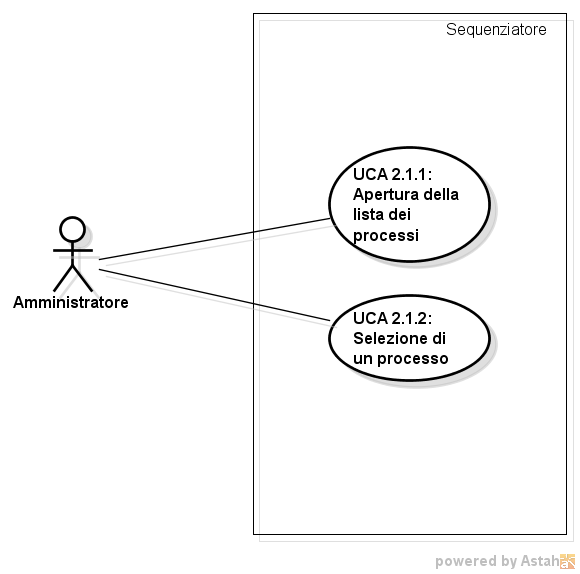
\includegraphics[trim=0cm 0.8cm 0cm 0cm,clip=true,width=%
\textwidth]
{./grafici/A21}
\caption{UCA 2.1: Scelta di un processo}
\end{figure}
\begin{itemize}
\item \textbf{Attori:} Amministratore;
\item \textbf{Descrizione:} L'amministratore può selezionare un processo da una lista o da i risultati di una ricerca;
\item \textbf{Precondizione:} L'amministratore vuole gestire un processo creato;
\item \textbf{Flusso principale degli eventi:}
\begin{enumerate}
\item L'amministratore può aprire la lista di processi;
\item L'amministratore può selezionare un processo.
\end{enumerate}
\item \textbf{Estensioni:} L'amministratore può effettuare la ricerca di un processo;
%\item \textbf{Inclusioni:}
\item \textbf{Postcondizione:} Il sistema è pronto per la gestione del processo scelto.
%\item \textbf{Scenario alternativo:}
\end{itemize}

\hypertarget{A2.1.1}{}
\bookmark[dest=A2.1.1,level=4]{UCA 2.1.1: Apertura della lista dei processi}
\subsubsection{UCA 2.1.1: Apertura della lista dei processi}
\begin{itemize}
\item \textbf{Attori:} Amministratore;
\item \textbf{Descrizione:} L'amministratore può aprire e visualizzare la lista dei processi;
\item \textbf{Precondizione:} L'amministratore vuole aprire la lista dei processi;
%\item \textbf{Scenario alternativo:}
%\item \textbf{Estensioni:}
\item \textbf{Postcondizione:} Il sistema ha visualizzato la lista dei processi creati dall'amministratore.
\end{itemize}

\hypertarget{A2.1.2}{}
\bookmark[dest=A2.1.2,level=4]{UCA 2.1.2: Selezione di un processo}
\subsubsection{UCA 2.1.2: Selezione di un processo}
\begin{itemize}
\item \textbf{Attori:} Amministratore;
\item \textbf{Descrizione:} L'amministratore può selezionare un processo dalla lista dei processi visualizzata;
\item \textbf{Precondizione:} L'amministratore sta visualizzando una lista di uno o più processi;
%\item \textbf{Scenario alternativo:}
%\item \textbf{Inclusioni:}
%\item \textbf{Estensioni:}
\item \textbf{Postcondizione:} Il sistema è pronto per la gestione del processo scelto.
\end{itemize}

\hypertarget{A2.1.3}{}
\bookmark[dest=A2.1.3,level=4]{UCA 2.1.3: Ricerca di un processo}
\subsubsection{UCA 2.1.3: Ricerca di un processo}
\begin{itemize}
\item \textbf{Attori:} Amministratore;
\item \textbf{Descrizione:} L'amministratore può ricercare un insieme di processi tra quelli creati;
\item \textbf{Precondizione:} L'amministratore vuole cercare un processo tra quelli creati;
%\item \textbf{Inclusioni:}
%\item \textbf{Estensioni:}
\item \textbf{Postcondizione:} Il sistema ha visualizzato la lista dei processi che soddisfano i criteri di ricerca.
\end{itemize}

\hypertarget{A2.2}{}
\bookmark[dest=A2.2,level=4]{UCA 2.2: Scelta degli utenti partecipanti}
\subsubsection{UCA 2.2: Scelta degli utenti partecipanti}
\begin{figure}[H]
\centering
\includegraphics[trim=0cm 0.8cm 0cm 0cm,clip=true,scale=0.75]%
{./grafici/A22}
\caption{UCA 2.2: Scelta degli utenti partecipanti}
\end{figure}
\begin{itemize}
\item \textbf{Attori:}
Amministratore;
\item \textbf{Descrizione:}
L'amministratore può scegliere gli utenti a cui permettere l'iscrizione al processo gestito;
\item \textbf{Precondizione:}
Il sistema ha aperto la pagina di gestione di un processo e l'amministratore vuole scegliere gli utenti che possono parteciparvi;
\item \textbf{Scenario principale:}
\begin{itemize}
\item L'amministratore può visualizzare la lista degli utenti registrati che non hanno il diritto di iscrizione al processo;
\item L'amministratore può aggiungere degli utenti a quelli che possono iscriversi al processo.
\end{itemize}
\item \textbf{Scenari alternativi:}
\begin{enumerate}
\item Non sono presenti utenti registrati senza diritto di iscrizione al processo, perciò il sistema rimane nello stato precedente.
\end{enumerate}
\item \textbf{Postcondizione:}
L'amministratore ha permesso a determinati utenti registrati l'iscrizione al processo gestito, e il sistema continua la gestione del processo.
\end{itemize}

\hypertarget{A2.2.1}{}
\bookmark[dest=A2.2.1,level=4]{UCA 2.2.1: Visualizzazione della lista degli utenti}
\subsubsection{UCA 2.2.1: Visualizzazione della lista degli utenti}
\begin{itemize}
\item \textbf{Attori:}
Amministratore;
\item \textbf{Descrizione:}
L'amministratore può visualizzare la lista degli utenti registrati al sistema che non hanno il diritto di iscrizione al processo gestito;
\item \textbf{Precondizione:}
L'utente vuole scegliere gli utenti a cui consentire il diritto di iscrizione al processo gestito;
\item \textbf{Postcondizione:}
Il sistema ha visualizzato la lista degli utenti registrati che non hanno il diritto di iscrizione al processo gestito, e può continuare la procedura di scelta degli utenti partecipanti.
\end{itemize}

\hypertarget{A2.2.2}{}
\bookmark[dest=A2.2.2,level=4]{UCA 2.2.2: Selezione degli utenti da aggiungere}
\subsubsection{UCA 2.2.2: Selezione degli utenti da aggiungere}
\begin{itemize}
\item \textbf{Attori:}
Amministratore;
\item \textbf{Descrizione:}
L'amministratore può selezionare uno o più utenti dalla lista visualizzata, per consentire loro l'iscrizione al processo gestito;
\item \textbf{Precondizione:}
L'utente sta visualizzando una lista di uno o più utenti, e vuole consentire ad alcuni di essi l'iscrizione al processo gestito;
\item \textbf{Postcondizione:}
Il sistema ha aggiunto il processo gestito alla lista dei processi disponibili degli utenti selezionati, e può continuare la procedura di scelta degli utenti partecipanti.
\end{itemize}

\hypertarget{A2.3}{}
\bookmark[dest=A2.3,level=4]{UCA 2.3: Consultazione di informazioni sull'esecuzione del processo}
\subsubsection{UCA 2.3: Consultazione di informazioni sull'esecuzione del processo}
\begin{figure}[H]
\centering
\includegraphics[trim=0cm 0.8cm 0cm 0cm,clip=true,scale=0.75]%
{./grafici/A23}
\caption{UCA 2.3: Consultazione di informazioni sull'esecuzione del processo}
\end{figure}
\begin{itemize}
\item \textbf{Attori:} Amministratore;
\item \textbf{Descrizione:}
L'amministratore può scegliere un processo precedentemente creato per recuperare informazioni sui suoi dati di creazione, sullo stato della sua esecuzione e su eventuali dati raccolti;
\item \textbf{Precondizione:}
Il sistema ha aperto la pagina di gestione di un processo;
\item \textbf{Scenario principale:}
\begin{itemize}
\item L'amministratore può recuperare le informazioni sui dati di creazione del processo;
\item L'amministratore può visualizzare lo stato del processo;
\item L'amministratore può consultare i dati ricevuti dagli utenti.
\end{itemize}
\item \textbf{Postcondizione:}
L'amministratore ha consultato le informazioni sul processo scelto e il sistema continua la sua gestione.
\end{itemize}

\hypertarget{A2.3.1}{}
\bookmark[dest=A2.3.1,level=4]{UCA 2.3.1: Recupero di informazioni sul processo}
\subsubsection{UCA 2.3.1: Recupero di informazioni sul processo}
\begin{itemize}
\item \textbf{Attori:}
Amministratore;
\item \textbf{Descrizione:}
L'amministratore può consultare le informazioni sul processo gestito. In particolare può visualizzare la descrizione del processo, i suoi criteri di terminazione, e i dati e le condizioni di superamento dei passi;
\item \textbf{Precondizione:}
L'amministratore vuole recuperare le informazioni generali sul processo gestito;
\item \textbf{Postcondizione:}
Il sistema ha visualizzato le informazioni generali sul processo gestito e continua la procedura di consultazione di informazioni.
\end{itemize}

\hypertarget{A2.3.2}{}
\bookmark[dest=A2.3.2,level=4]{UCA 2.3.2: Visualizzazione dello stato del processo}
\subsubsection{UCA 2.3.2: Visualizzazione dello stato del processo}
\begin{figure}[H]
\centering
\includegraphics[trim=0cm 0.8cm 0cm 0cm,clip=true,scale=0.75]%
{./grafici/A232}
\caption{UCA 2.3.2: Visualizzazione dello stato del processo}
\end{figure}
\begin{itemize}
\item \textbf{Attori:}
Amministratore;
\item \textbf{Descrizione:}
L'amministratore può visualizzare il numero di utenti iscritti al processo e il numero di utenti che lo hanno completato;
\item \textbf{Precondizione:}
L'amministratore vuole visualizzare lo stato del processo gestito;
\item \textbf{Scenario principale:}
\begin{itemize}
\item L'amministratore può visualizzare il numero di utenti iscritti al processo gestito;
\item L'amministratore può visualizzare il numero di utenti che hanno completato il processo gestito.
\end{itemize}
\item \textbf{Postcondizione:}
Il sistema ha visualizzato le informazioni sullo stato del processo gestito e continua la procedura di consultazione di informazioni.
\end{itemize}

\hypertarget{A2.3.2.1}{}
\bookmark[dest=A2.3.2.1,level=4]{UCA 2.3.2.1: Visualizzazione del numero di utenti iscritti}
\subsubsection{UCA 2.3.2.1: Visualizzazione del numero di utenti iscritti}
\begin{itemize}
\item \textbf{Attori:}
Amministratore;
\item \textbf{Descrizione:}
L'amministratore può visualizzare il numero di utenti iscritti al processo gestito;
\item \textbf{Precondizione:}
L'amministratore vuole visualizzare lo stato del processo gestito;
\item \textbf{Postcondizione:}
Il sistema ha visualizzato il numero di utenti iscritti al processo gestito e continua la visualizzazione dello stato del processo.
\end{itemize}

\hypertarget{A2.3.2.2}{}
\bookmark[dest=A2.3.2.2,level=4]{UCA 2.3.2.2: Visualizzazione del numero di completamenti}
\subsubsection{UCA 2.3.2.2: Visualizzazione del numero di completamenti}
\begin{itemize}
\item \textbf{Attori:}
Amministratore;
\item \textbf{Descrizione:}
L'amministratore può visualizzare il numero di utenti che hanno completato il processo gestito;
\item \textbf{Precondizione:}
L'amministratore vuole visualizzare lo stato del processo gestito;
\item \textbf{Postcondizione:}
Il sistema ha visualizzato il numero di utenti che hanno completato il processo gestito e continua la visualizzazione dello stato del processo.
\end{itemize}

\hypertarget{A2.3.3}{}
\bookmark[dest=A2.3.3,level=4]{UCA 2.3.3: Consultazione dei dati ricevuti}
\subsubsection{UCA 2.3.3: Consultazione dei dati ricevuti}
\begin{itemize}
\item \textbf{Attori:} Amministratore;
\item \textbf{Descrizione:}
L'amministratore può consultare i dati inviati dagli utenti al sistema che hanno comportato il superamento di un passo;
\item \textbf{Precondizione:}
Il sistema ha aperto la pagina di gestione di un processo e vuole consultare i dati inviati dagli utenti;
\item \textbf{Postcondizione:}
Il sistema ha visualizzato i dati ricevuti dagli utenti e continua la procedura di consultazione di informazioni.
\end{itemize}

\hypertarget{A2.4}{}
\bookmark[dest=A2.4,level=4]{UCA 2.4: Controllo dei dati che richiedono approvazione}
\subsubsection{UCA 2.4: Controllo dei dati che richiedono approvazione}
\begin{figure}[H]
\centering
\includegraphics[trim=0cm 0.8cm 0cm 0cm,clip=true,scale=0.75]%
{./grafici/A24}
\caption{UCA 2.4: Controllo dei dati che richiedono approvazione}
\end{figure}
\begin{itemize}
\item \textbf{Attori:}
Amministratore;
\item \textbf{Descrizione:}
L'amministratore può permettere l'avanzamento eventuali passi che richiedono l'approvazione dei dati inviati dall'utente.
Il responso dell'attività di controllo viene inviato all'utente che potrà visualizzare l'esito del passo e continuare la procedura di esecuzione del passo;
\item \textbf{Precondizione:}
Il sistema ha aperto la pagina di gestione di un processo in cui esiste almeno un insieme di dati inviati al sistema che richiedono il controllo dell'amministratore;
\item \textbf{Flusso principale degli eventi:}
\begin{enumerate}
\item L'amministratore può consultare le informazioni inviate dagli utenti che richiedono la sua approvazione;
\item L'amministratore può inviare l'esito del controllo di uno o più dati consultati.
\end{enumerate}
\item \textbf{Postcondizione:}
Il sistema ha eseguito e salvato le operazioni effettuate dall'amministratore sui dati che richiedevano approvazione.
\end{itemize}

\hypertarget{A2.4.1}{}
\bookmark[dest=A2.4.1,level=4]{UCA 2.4.1: Consultazione delle informazioni ricevute}
\subsubsection{UCA 2.4.1: Consultazione delle informazioni ricevute}
\begin{itemize}
\item \textbf{Attori:}
Amministratore;
\item \textbf{Descrizione:}
L'amministratore può consultare le informazioni testuali, numeriche, geografiche, temporali e le immagini inviate dagli utenti, relative ad un passo che richiede l'approvazione manuale per essere superato;
\item \textbf{Precondizione:}
L'amministratore vuole consultare le informazioni inviate dagli utenti che richiedono approvazione, relative al processo gestito;
\item \textbf{Postcondizione:}
Il sistema ha visualizzato le informazioni inviate dagli utenti che richiedono l'approvazione dell'amministratore, e continua la procedura di controllo dei dati ricevuti.
\end{itemize}

\hypertarget{A2.4.2}{}
\bookmark[dest=A2.4.2,level=4]{UCA 2.4.2: Invio dell'esito del controllo}
\subsubsection{UCA 2.4.2: Invio dell'esito del controllo}
\begin{figure}[H]
\centering
\includegraphics[trim=0cm 0.8cm 0cm 0cm,clip=true,scale=0.75]%
{./grafici/A242}
\caption{UCA 2.4.2: Invio dell'esito del controllo}
\end{figure}
\begin{itemize}
\item \textbf{Attori:}
Amministratore;
\item \textbf{Descrizione:}
L'amministratore può decidere di approvare o respingere i dati ricevuti da un utente che richiedono approvazione.
Il responso dell'attività di controllo viene inviato all'utente che potrà visualizzare l'esito del passo e continuare la procedura di esecuzione del passo;
\item \textbf{Precondizione:}
L'amministratore ha consultato le informazioni inviate dagli utenti che richiedono approvazione e vuole inviare l'esito del controllo;
\item \textbf{Scenario principale:}
\begin{itemize}
\item L'amministratore può approvare i dati ricevuti;
\item L'amministratore può richiedere la ripetizione del passo.
\end{itemize}
\item \textbf{Postcondizione:}
L'esito del controllo è stato notificato all'utente e il sistema continua la procedura di controllo dei dati ricevuti.
\end{itemize}

\hypertarget{A2.4.2.1}{}
\bookmark[dest=A2.4.2.1,level=4]{UCA 2.4.2.1: Approvazione dei dati}
\subsubsection{UCA 2.4.2.1: Approvazione dei dati}
\begin{itemize}
\item \textbf{Attori:}
Amministratore;
\item \textbf{Descrizione:}
L'amministratore può scegliere di approvare i dati ricevuti da un utente. Il sistema notifica la decisione dell'amministratore all'utente, che può concludere il passo in corso;
\item \textbf{Precondizione:}
L'amministratore ha consultato le informazioni inviate dagli utenti e vuole approvarle;
\item \textbf{Postcondizione:}
Il sistema notifica all'utente l'esito positivo del controllo, è pronto per consentire all'utente la conclusione del passo, e continua la procedura di controllo dei dati ricevuti.
\end{itemize}

\hypertarget{A2.4.2.2}{}
\bookmark[dest=A2.4.2.2,level=4]{UCA 2.4.2.2: Richiesta ripetizione del passo}
\subsubsection{UCA 2.4.2.2: Richiesta ripetizione del passo}
\begin{itemize}
\item \textbf{Attori:}
Amministratore;
\item \textbf{Descrizione:}
L'amministratore può scegliere di respingere i dati ricevuti da un utente. Il sistema notifica la decisione dell'amministratore all'utente, che può rieseguire il passo in corso e modificare i dati da inviare;
\item \textbf{Precondizione:}
L'amministratore ha consultato le informazioni inviate dagli utenti e vuole respingerle;
\item \textbf{Postcondizione:}
Il sistema notifica all'utente l'esito negativo del controllo, consente all'utente il reinserimento dei dati, e continua la procedura di controllo dei dati ricevuti.
\end{itemize}

\hypertarget{A2.5}{}
\bookmark[dest=A2.5,level=4]{UCA 2.5: Terminazione del processo}
\subsubsection{UCA 2.5: Terminazione del processo}
\begin{itemize}
\item \textbf{Attori:} Amministratore;
\item \textbf{Descrizione:}
L'amministratore può terminare forzatamente il processo gestito. Gli utenti iscritti al processo non potranno più eseguirne i passi, ma potranno svolgere le funzionalità di conclusione del processo;
\item \textbf{Precondizione:}
L'amministratore vuole terminare il processo gestito;
\item \textbf{Postcondizione:}
Il processo gestito è terminato. L'amministratore può eliminarlo e gli utenti iscritti ad esso possono svolgere le funzionalità di conclusione del processo.
\end{itemize}

\hypertarget{A2.6}{}
\bookmark[dest=A2.6,level=4]{UCA 2.6: Eliminazione del processo}
\subsubsection{UCA 2.6: Eliminazione del processo}
\begin{itemize}
\item \textbf{Attori:} Amministratore;
\item \textbf{Descrizione:}
L'amministratore può eliminare un processo dall'insieme dei processi creati.
Può eliminare un processo terminato forzatamente o al verificarsi dei criteri di terminazione.
Il processo eliminato non sarà più accessibile e gestibile dall'amministratore, ma sarà accessibile agli utenti iscritti ad esso, se non l'hanno ancora chiuso, per svolgere le funzionalità di conclusione del processo;
\item \textbf{Precondizione:}
Il processo gestito è terminato, e l'amministratore vuole eliminarlo;
\item \textbf{Postcondizione:}
Il processo gestito non è più accessibile dall'amministratore. Gli utenti iscritti ad esso che non lo hanno ancora chiuso, possono svolgere le funzionalità di conclusione del processo.
\end{itemize}